\documentclass[draft]{scrartcl}
\title{Simplicial Homology}
\author{Jan Zwank}
\usepackage{amsmath,amssymb,amsthm}
\usepackage[utf8]{inputenc}
\usepackage[T1]{fontenc}
\usepackage{hyperref,microtype,lmodern,csquotes}
\usepackage[english]{babel}
\usepackage{tikz, tikz-cd}
\usetikzlibrary{3d,calc,decorations}
\usepackage{pst-solides3d}
\usepackage{caption}

\theoremstyle{plain}
\newtheorem{theorem}{Theorem}[section]
\newtheorem{lemma}[theorem]{Lemma}
\newtheorem{korollar}[theorem]{Korollar}
\newtheorem{satz}[theorem]{Satz}
\newtheorem{hilfssatz}[theorem]{Hilfssatz}
\newtheorem{corollary}[theorem]{Corollary}

\theoremstyle{definition}
\newtheorem	{definition}[theorem]{Definition}
\newtheorem{beispiel}[theorem]{Beispiel}
\newtheorem{beispiele}[theorem]{Beispiele}
\newtheorem{konvention}[theorem]{Konvention}
\newtheorem{notation}[theorem]{Notation}
\newtheorem{axiom}[theorem]{Axiom}
\newtheorem{example}[theorem]{Example}
\newtheorem{examples}[theorem]{Examples}

\theoremstyle{remark}
\newtheorem*{bemerkung}{Bemerkung}
\newtheorem*{bemerkungen}{Bemerkungen}
\newtheorem*{frage}{Frage}

\usetikzlibrary{decorations.markings,intersections}
\tikzset{->-/.style={decoration={
			markings,
			mark=at position #1 with {\arrow[line width=3pt]{stealth}}},postaction={decorate}}}

\newcommand{\SH}{Simplicial Homology}
\newcommand{\sh}{simplicial homology}
\newcommand{\Z}{\mathbb{Z}}
\newcommand{\Sp}{\mathbb{S}}
\newcommand{\im}{\mathrm{Im}\,}
\newcommand{\qandq}{\quad \text{and} \quad}
\newcommand{\qqandqq}{\qquad \text{and} \qquad}
\newcommand{\scs}{simplicial complexes}
\usepackage%[style=authoryear]
	{biblatex}
\bibliography{bibliography}
\begin{document}
	\maketitle
	
	\begin{abstract}
		%TODO 
		Abstract goes here
	\end{abstract}
\tableofcontents

\clearpage

\section{Motivation}\label{motivation}
One of the main goals when studying (topological) spaces (or in this case \scs) is to determine whether two spaces are homotopic
%TODO homeomorphic?
 or not. The first method that is often applied is to check if both spaces are simply connected. A more advanced approach checks not only simply connectedness but also if the fundamental groups $\pi_1$ coincide\footnote{If $X$ is a simply connected space then $\pi_1(X)=0$. Furthermore, the fundamental group is homotopy invariant (up to isomorphism), so homotopic spaces have isomorphic fundamental groups. A more precise formulation of this statement can be found in Hatchers book \parencite[Prop. 1.18, p. 37]{ha}:
\begin{quotation}
	\begin{quote}
		If $\phi: X\to Y$ is a homotopy equivalence, then the induces homomorphism $\phi_*:\pi_1(X,x_0)\to\pi_1(Y,\phi(x_0))$ is an isomorphism for all $x_0\in X$.
	\end{quote}
\end{quotation} }.

It turns out that this is a valuable tool for one and two dimensional \scs. But this method fails for complexes with cells in higher dimensions. It can be shown that the fundamental group actually only depends on the 2-skeleton of the complex \cite[vgl.][p. 173]{ar}. 

Even though this method can be generalized to the study of higher homotopy groups $\pi_n$, this is often more difficult than necessary since the computation of those groups is far from trivial.

In the following we will explore the concept of \sh{} groups and how it can be used to classify spaces. We will see that they allow us to tackle the problem of deciding whether two \textbf{polyhedra}\footnote{A polyhedron is the polytope of a simplicial complex.} are homeomorphic, since simplicial homology is only defined on such spaces. However, the concept of \sh{} can be generalized to singular homology, which can be applied to a broader category of spaces and coincides with \sh{} if both are defined.

However, singular homology groups will not be covered here. The interested reader might refer to the book of Munkres \cite{mu} or Hatcher \cite{ha} to learn more about singular homology groups.

When we concern ourselfes with the question how closed paths on the torus are different from those on the sphere, we can notice the following:

Any Jordan curve (i.e. nonselfintersecting, closed path) on a sphere divides the surface into two \glqq regions\grqq{} as depicted in \autoref{divided-sphere}\footnote{For a more precise statement see \url{https://en.wikipedia.org/wiki/Jordan_curve_theorem}}. The same is not true for the torus. In \autoref{path-on-torus} we see that even tough there are Jordan curves on a torus that bound a \glqq region\grqq of the surface, not all Jordan curves have that property \cite[p. 173f][see]{ar}.

%While we considered all possible paths when we were talking about the fundamental group we will now only consider those that aren't the boundary of a portion of the surface. A great motivation for this approach is given by Armstrong \cite[p. 173f]{ar}:

%Any closed path on the 2-sphere divides the surface into two regions as shown in \autoref{divided-sphere}\footnote{For a more precise statement see \url{https://en.wikipedia.org/wiki/Jordan_curve_theorem}}.

\begin{figure}[h]
	
\parbox{\linewidth}{\parbox[t]{.5\linewidth}{\centering
	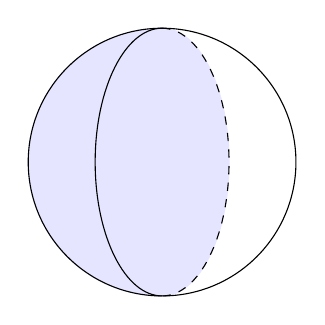
\begin{tikzpicture}[scale=1.7]
		%\draw (-1,0) arc (180:360:1cm and 0.5cm);
		%\draw[dashed] (-1,0) arc (180:0:1cm and 0.5cm);
		\filldraw[blue!10] (0,1)  arc (90:270:1cm) arc (-90:90:0.5cm and 1cm);
		\draw (0,1) arc (90:270:0.5cm and 1cm);
		\draw[dashed] (0,1) arc (90:-90:0.5cm and 1cm);
		\draw (0,0) circle (1cm);
		%\shade[ball color=blue!10!white,opacity=0.20] (0,0) circle (1cm);
	\end{tikzpicture}}%
\parbox[t]{.5\linewidth}{\centering
	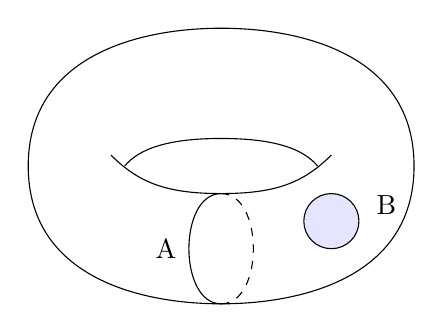
\begin{tikzpicture}[scale=0.7]
	\draw (-3.5,0) .. controls (-3.5,2) and (-1.5,2.5) .. (0,2.5);
	\draw[xscale=-1] (-3.5,0) .. controls (-3.5,2) and (-1.5,2.5) .. (0,2.5);
	\draw[rotate=180] (-3.5,0) .. controls (-3.5,2) and (-1.5,2.5) .. (0,2.5);
	\draw[yscale=-1] (-3.5,0) .. controls (-3.5,2) and (-1.5,2.5) .. (0,2.5);
	
	\draw (-2,.2) .. controls (-1.5,-0.3) and (-1,-0.5) .. (0,-.5) .. controls (1,-0.5) and (1.5,-0.3) .. (2,0.2);
	
	\draw (-1.75,0) .. controls (-1.5,0.3) and (-1,0.5) .. (0,.5) .. controls (1,0.5) and (1.5,0.3) .. (1.75,0);
	
	\draw (0,-0.5) to [out=180, in=180](0,-2.5);
	\draw[dashed] (0,-2.5) to [out=0, in=0](0,-0.5);
	\draw (-1,-1.5) node{A};
	\draw[fill=blue!10!white] (2,-1) circle (0.5);
	\draw (3,-.7) node{B};
	\end{tikzpicture}
%\begin{pspicture}(-6,-4)(6,4)
%\psset{viewpoint=30 0 15 rtp2xyz,Decran=30,lightsrc=viewpoint}
%\psSolid[object=tore,r1=2.5,r0=.7,ngrid=36 72,fillcolor=blue!10!white,grid=false]%
%\end{pspicture}
}}
\parbox[t]{.5\linewidth}{\captionsetup{width=.9\linewidth}
\caption{Any closed path on the sphere divides the surface into two regions.\label{divided-sphere} }}%
\parbox[t]{.5\linewidth}{\captionsetup{width=.9\linewidth}
\caption{There are closed paths on the torus that do not divide the surface into two regions.\label{path-on-torus}}}

\end{figure}

\section{\SH{} Groups with Integer Coefficients}\label{first-hom}

We will use the following definition by Munkres \cite[p. 26]{mu} %and Armstrong \cite[p. 174]{ar}:
\begin{definition}
	For a simplex $\sigma$ we say that two orderings of its vertex set are equivalent if they differ by an even permutation. For a simplex with nonzero dimension, the orderings of the vertices fall into two equivalence classes, called the \textbf{orientations} of $\sigma$. An \textbf{oriented simplex} is a simplex together with an orientation.
\end{definition}
Further we will use the same notation as Munkres \cite[p. 26]{mu}
\begin{notation}
	For geometrically independent points $v_0,\dots,v_p$ we denote the simplex they span with
	\[
	[v_0,\dots,v_p].
	\]
	For an oriented simplex we will use the notation
	\[
	(v_0,\dots,v_p).
	\]
	where the orientation is given by this particular ordering.
%	A change in orientation will be denoted by a minus sign. So, for example
%	\[
%	(v_1,v_2,v_3)=(v_2,v_3,v_1)=(v_3,v_1,v_2)=-(v_1,v_3,v_2)=-(v_2,v_1,v_3)=-(v_3,v_2,v_1)
%	\]
\end{notation}

A choice of orientation is usually depicted with arrows as can be seen in \autoref{orientation-arrows}

\begin{figure}
	\centering

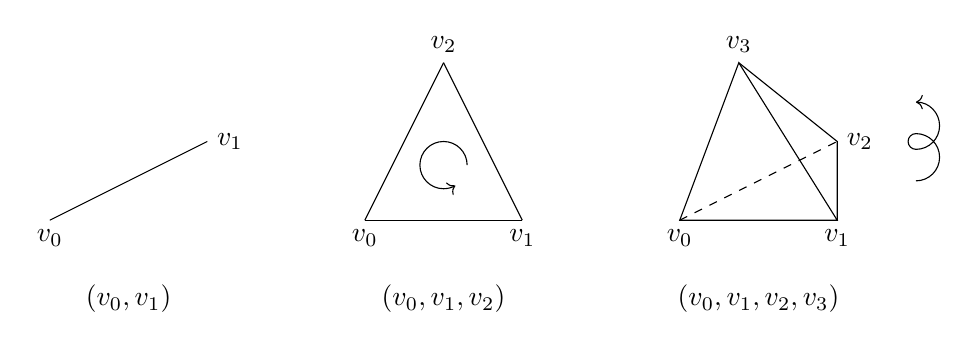
\begin{tikzpicture}
	\draw[] (0,0) node[below]{$v_0$}->(1,0.5);
	\draw (1,0.5)-- (2,1) node[right]{$v_1$};
	\draw (1,-1) node{$(v_0,v_1)$};
	%
	\draw[] (4,0) node[below]{$v_0$}--(6,0)node[below]{$v_1$};
	\draw[] (6,0) -- (5,2) node[above]{$v_2$};
	\draw[] (5,2)--(4,0);
	\draw (5,-1) node{$(v_0,v_1,v_2)$};	
	\draw[->] (5.3,0.7)arc[start angle=0, end angle=300,radius=0.3cm];
	%
	\draw (8,0) node[below]{$v_0$}--(10,0)node[below]{$v_1$}--(8.75,2)node[above]{$v_3$}--cycle;
	\draw (10,0)--(10,1)node[right]{$v_2$}--(8.75,2);
	\draw[dashed] (8,0)--(10,1);
	\draw (9,-1) node{$(v_0,v_1,v_2,v_3)$};
	\draw[->] (11,0.5) arc[start angle=-90, end angle=90, radius=0.3cm] arc [start angle=90, end angle=270,radius=0.1] arc[start angle=-90, end angle=90, radius=0.3];
\end{tikzpicture}
\caption{Indicating orientation with arrows \cite[see][p.27]{mu}\label{orientation-arrows}}
\end{figure}
%
%\begin{definition}
%	The boundary operator of the oriented edge $[v_0,v_1]$ is defined to be the formal linear combination of points
%	\[
%	\partial[v_0,v_1]=v_1-v_0
%	\]
%	and the boundary of the oriented triangle $[v_0,v_1,v_2]$ is defined to be the formal linear combination of edges
%	\[
%	\partial[v_0,v_1,v_2]=[v_1,v_2]-[v_0,v_2]+[v_0,v_1]
%	\]
%\end{definition}
%
%We see that for the closed curve $B$ from \autoref{path-on-torus} with a triangularization as depicted in \autoref{closed-curve} has vanishing boundary, since
%\[
%\partial(a+b+c)=\partial[v_0,v_1]+\partial[v_1,v_2]+\partial[v_2,v_0]=(v_1-v_0)+(v_2-v_1)+(v_0-v_2)=0
%\]
%
%Further, we see that $B$ is indeed the boundary of the interior region, since
%\[
%\partial[v_0,v_1,v_2]=[v_1,v_2]-[v_0,v_2]+[v_0,v_1]=a+b+c
%\]
%
%\begin{figure}\centering
%	\begin{tikzpicture}[scale=2]
%		\draw[fill=blue!10](0,0)--(1,1)--(2,0)--(0,0);
%		\draw node[left]{$v_0$};
%		\draw[->] (0,0)--(0.5,0.5) node[left]{$a$};
%		\draw(0.5,0.5)--(1,1)node[above]{$v_1$};
%		\draw[->](1,1)--(1.5,0.5) node[right]{$b$};
%		\draw (1.5,0.5)--(2,0) node[right]{$v_2$};
%		\draw[->] (2,0)--(1,0) node[below]{$c$};
%		\draw (2,0)--(0,0) node[left]{$v_0$};
%	\end{tikzpicture}
%	\caption{A closed curve triangulated as $[v_0,v_1,v_2]$.\label{closed-curve}}
%\end{figure}
%
%We will now construct the abelian group $Z_1(K)$ by considering all those formal linear combinations of edges with integer coefficients (for now) that satisfy the condition of a vanishing boundary. We  call $Z_1(K)$ the group of 1-cycles.
%
%Similarly, we say that a 1-cycle is a bounding cycle if we can find a linear combination of triangles whose boundary  is the given cycle. The group of such bounding cycles shall be denoted by $B_1(K)$.
%
%Thinking back to the motivational part of this section, we are only \glqq interested \grqq{} in the 1-cycles that aren't also bounding cycles. Obviously, $B_1(K)$ is a subgroup of $Z_1(K)$, so we can form the quotient group
%\[
%H_1(K)=Z_1(K)/B_1(K).
%\]
%This is called the first homology group of $K$.%TODO I never stated what K is.
%
%
%Nowhere in \autoref{first-hom} where we restricted to two dimensions. Actually, the computation of higher simplicial homology groups is very similar to that in 2-dimensions.
%
%We begin with the following definition from Munkres \cite{mu}

To define simplicial homology groups in any meaningful way, we need a few definitions that allow us to formulate our ideas form \autoref{motivation} more precise. There are several ways to go about this with various amounts of rigor. In this paper, we will follow the path of Munkres \cite[p. 27f]{mu}.

%TODO This is a direct citation. Do I need to state that any further?
\begin{definition}\label{def-chain}
	Let $K$ be a simlicial complex. A \textbf{$p$-chain} on $K$ is a function $c$ from the set of oriented $p$-simplices of $K$ to the integers such that:
	\begin{enumerate}
		\item $c(\sigma)=-c(\sigma^\prime)$ if $\sigma$ and $\sigma^\prime$ are opposite orientations of the same simplex.
		\item $c(\sigma)=0$ for all but finitely many oriented $p$-simplices $\sigma$.
	\end{enumerate}
We add $p$-chains by adding their values; the resulting group is denoted $C_p(K)$ and is called the group of (oriented) $p$-chains of $K$. If $p<0$ or $p>\dim K$, we let $C_p(K)$ denote the trivial group.

If $\sigma$ is an oriented simplex, the elementary chain $c_\sigma$ corresponding to $\sigma$ is the function defined as follows:
\begin{align*}c_\sigma(\sigma)=&1,\\
 c_\sigma(\sigma^\prime)=&-1&&\text{ if $\sigma^\prime$ is the opposite orientation of $\sigma$}\\
 c_\sigma(\tau)=&0 &&\text{ for all other oriented simplices $\tau$.} 
 \end{align*}
\end{definition}

It is common practice to to abuse the notation here. If clear by context we use the symbol $\sigma$ not only to denote the (oriented) simplex, but also the corresponding elementary chain.

We are now able to formulate the our first result as can be found in Munkres book \cite[Lemma 5.1, p. 28]{mu}:
\begin{lemma}
	$C_p(K)$ is free abelian; a basis for $C_p(K)$ can be obtained by orienting each $p$-simplex and using the corresponding elementary chains as a basis.
\end{lemma}

\begin{proof}
	It is easy to see that each chain $c$ in $C_p(K)$ can be expressed uniquely as a linear combination of the elementary chains $c_{\sigma_i}$ of the simplices of $K$, i.e.
	\[
	c=\sum_{i}n_i c_{\sigma_i}.
	\]
	Here, the the chain $c$ assigns the value $n_i$ to each simplex $\sigma_i$, $-n_i$ for the simplex $\sigma_i$ with reversed orientation and $0$ to every simplex that does not appear in the summation.\footnote{Recall that by definition of the elementary chains we have \[c_{\sigma_i}(\tau)=\begin{cases}
		1 &\text{if }\sigma_i=\tau\\
		-1&\text{if }\tau \text{ is the opposite orientation of }\sigma_i\\
		0&\text{else}
		\end{cases}
		\]}
\end{proof}

\begin{definition}
	We define the boundary operator 
	\[
	\partial_p:\quad C_p(K)\to C_{p-1}(K)
	\]
	to be the homomorphism via its action on an oriented simplex $\sigma=(v_0,\dots,v_p)$:
	\[
	\partial_p\sigma=\partial_p(v_0,\dots,v_p)=\sum_{i=0}^{p}(-1)^i(v_0,\dots,\hat{v}_i,\dots,v_p)
	\]
	where the symbol $\hat{v}_i$ means that the vertex $v_i$ is to be deleted from the array.
\end{definition}

As the name suggests, the result of this homomorphism indeed refers to the (topological) boundary of the simplex once we interpret the sum of two elementary chains as the union of the corresponding simplices as we will see in the several examples, but first we have to check well-definedness. For that, it is necessary to show that
\[\partial_p(-\sigma)=-\partial_p(\sigma) 
\]
Since the orientation fo a simplex only depends on the \emph{sign} of the permutation, it is sufficient to check for the simple case of exchanging $v_0$ and $v_1$:

\begin{align*}
	&\partial_p(v_0,\dots,v_p)+\partial_p(v_1,v_0,v_2,\dots,v_p)\\
	=&(v_1,\dots,v_p)-(v_0,v_2,\dots,v_p)+\sum_{i=2}^{p}(-1)^i(v_0,\dots,\hat{v}_i,\dots,v_p)\\
	+&(v_0,v_2,\dots,v_p)-(v_1,v_2,\dots,v_p)+\sum_{i=2}^p(-1)^i\underset{=-(v_0,v_1,v_2,\dots,\hat{v}_i,\dots,v_p)}{\underbrace{\ensuremath{(v_1,v_0,v_2,\dots,\hat{v}_i,\dots,v_p)}}}=0
\end{align*}

\begin{examples}\mbox{}
	\begin{enumerate}
		\item \parbox[c]{.5\linewidth}{$\partial_1(v_0,v_1)=v_1-v_0$}%
		\parbox[c]{.5\linewidth}{
		\begin{tikzpicture}
		\draw[->] (0,0) node[below]{$v_0$}->(1,0.5);
		\draw (1,0.5)-- (2,1) node[right]{$v_1$};
		%
		\draw[fill=black](4,.5)circle (1pt) node[below]{$v_1$};
		\draw[fill=black](5,.5)circle (1pt) node[below]{$v_0$};
		\draw (4.5,.5) node{$-$};
		\end{tikzpicture}}
	\item 
	\parbox[c]{.5\linewidth}{$\partial_2(v_0,v_1,v_2)=(v_1,v_2)-(v_0,v_2)+(v_0,v_1)$}%
	\parbox[c]{.5\linewidth}{
		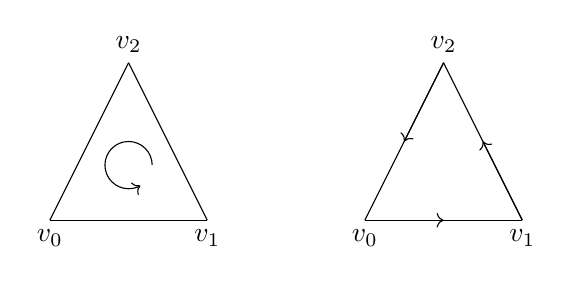
\begin{tikzpicture}
			\draw[] (4,0) node[below]{$v_0$}--(6,0)node[below]{$v_1$};
			\draw[] (6,0) -- (5,2) node[above]{$v_2$};
			\draw[] (5,2)--(4,0);
			%\draw (5,-1) node{$(v_0,v_1,v_2)$};	
			\draw[->] (5.3,0.7)arc[start angle=0, end angle=300,radius=0.3cm];
			%
			\draw[] (8,0) node[below]{$v_0$}--(10,0)node[below]{$v_1$};
			\draw[] (10,0) -- (9,2) node[above]{$v_2$};
			\draw[] (9,2)--(8,0);
			\draw[->](8,0)--(9,0);
			\draw[->](10,0)--(9.5,1);
			\draw[->](9,2)--(8.5,1);
		\end{tikzpicture}
	}
	\item 
	\parbox[c]{.5\linewidth}{\begin{align*}\partial_3(v_0,v_1,v_2,v_3)&=(v_1,v_2,v_3)-(v_0,v_2,v_3)\\
	&+(v_0,v_1,v_3)-(v_0,v_1,v_2)
	\end{align*}}%
\parbox[c]{.5\linewidth}{ 
	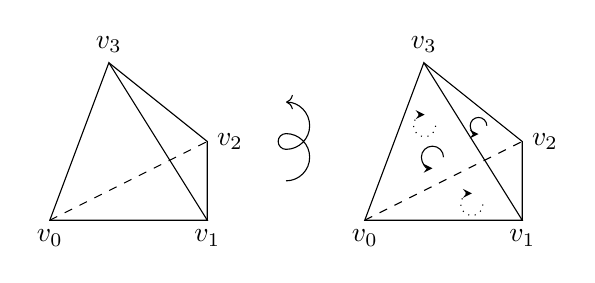
\begin{tikzpicture}
		\draw (0,0) node[below]{$v_0$}--(2,0)node[below]{$v_1$}--(0.75,2)node[above]{$v_3$}--cycle;
		\draw (2,0)--(2,1)node[right]{$v_2$}--(0.75,2);
		\draw[dashed] (0,0)--(2,1);
		\draw[->] (3,0.5) arc[start angle=-90, end angle=90, radius=0.3cm] arc [start angle=90, end angle=270,radius=0.1] arc[start angle=-90, end angle=90, radius=0.3];
		%
		\draw (4,0) node[below]{$v_0$}--(6,0)node[below]{$v_1$}--(4.75,2)node[above]{$v_3$}--cycle;
		\draw (6,0)--(6,1)node[right]{$v_2$}--(4.75,2);
		\draw[dashed] (4,0)--(6,1);
		%
		\draw[->,>=stealth](5.55,1.2)arc[start angle=0,end angle=270,radius=3pt];
		\draw[->,>=stealth,dotted](4.9,1.2)arc[start angle=0,end angle=-270,radius=4pt];
		\draw[->,>=stealth](5,.8)arc[start angle=0,end angle=270,radius=4pt];
		\draw[->,>=stealth,dotted](5.5,.2)arc[start angle=0,end angle=-270,radius=4pt];
	\end{tikzpicture}
	}

	\end{enumerate}
	
\end{examples}

We will now consider the following diagram. (For the sake of readability, we deleted the dimension subscripts from the boundary operator)
\begin{center}
\begin{tikzcd}
	C_\bullet:&\cdots \arrow[r, "\partial"] & C_{p+1}\arrow[r,"\partial"]&C_p\arrow[r,"\partial"]&C_{p-1}\arrow[r,"\partial"]&\cdots \\
\end{tikzcd}

\end{center}

\begin{lemma}
	$C_\bullet$ is a chain complex.
\end{lemma}

\begin{proof}
	We need to show that $\partial_{p-1}\circ\partial_p\equiv 0$. It is not hard to prove this, it just requires a lot of bookkeeping:
	
	Let $\sigma=(v_0,\dots,v_p)$ be an arbitrary $p$-chain, then
	\begin{align*}
		\partial_{p-1}\circ\partial_p(\sigma)&=\partial_{p-1}\left(\sum_{i=0}^{p}(-1)^i(v_0,\dots,\hat{v}_i,\dots,v_p)\right)=\sum_{i=0}^{p}(-1)^i\partial_{p-1}(v_0,\dots,\hat{v}_i,\dots,v_p)\\
		&=\sum_{i=0}^{p}(-1)^i\sum_{\parbox{.8cm}{\centering\scriptsize
				$j=0$\\$j\neq i$}}^{p}(-1)^j(v_0,\dots,\hat{v}_j,\dots,\hat{v}_i,\dots,v_p)
	\end{align*}
	Each of these term shows up twice with different signs. Thus, everything cancels.

\end{proof}

A common question for chain complexes is exactness. As we will see later in this chapter, they will only be exact for special cases. 

Before we define the simplicial homology groups, we will introduce one more definition:

\begin{definition}\mbox{}
	\begin{enumerate}
		\item The kernel of $\partial_p: C_p(K)\to C_{p-1}(K)$ is called the group of $p$-cycles and denoted by $Z_p(K)$.
		\item The immage of $\partial_{p+1}: C_{p+1}(K)\to C_{p}(K)$ is called the group of $p$-boundaries and is denoted $B_p(K)$.
	\end{enumerate}
	
\end{definition}
The previous lemma states that $B_p(K)\subset Z_p(K)$.

Let us remind ourselves of what we wanted to do in \autoref{motivation}. We wanted to consider those curves (\emph{cycles}) that were not the \emph{boundary} of some part of the surface. With this in mind, we can now state the definition of simplical homology groups

\begin{definition}
	We define \[
	H_p(K):=Z_p(K)/B_p(K)=\ker \partial_p/\im \partial_{p+1}
	\]
	and call it the \textbf{$\mathbf{p}$-th simplicial homology goup of $\mathbf{K}$}.
\end{definition}
%TODO Examples

\begin{examples}\mbox{}
	\begin{enumerate}
		\item Lets start with a simple triangulation\footnote{A triangulation of a space $T$ is a simplicial complex $X$ whose geometric realization $|X|$ is homeomorphic to $T$.}
		 of $\Sp^2$ like the hollow tetrahedron (depicted in \autoref{hollow-tetrahedron}) \[X=\langle v_0v_1v_2,v_0v_1v_3,v_0v_2v_3,v_1v_2v_3 \rangle. \]
			 	
		 	\begin{figure}\centering
		 		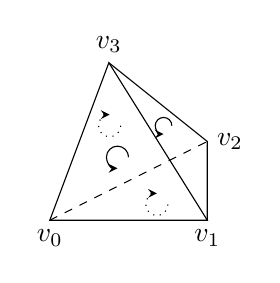
\begin{tikzpicture}
		 		\draw (4,0) node[below]{$v_0$}--(6,0)node[below]{$v_1$}--(4.75,2)node[above]{$v_3$}--cycle;
		 		\draw (6,0)--(6,1)node[right]{$v_2$}--(4.75,2);
		 		\draw[dashed] (4,0)--(6,1);
		 			\draw[->,>=stealth](5.55,1.2)arc[start angle=0,end angle=270,radius=3pt];
		 			\draw[->,>=stealth,dotted](4.9,1.2)arc[start angle=0,end angle=-270,radius=4pt];
		 			\draw[->,>=stealth](5,.8)arc[start angle=0,end angle=270,radius=4pt];
		 			\draw[->,>=stealth,dotted](5.5,.2)arc[start angle=0,end angle=-270,radius=4pt];
		 		\end{tikzpicture}
		 		\caption{geometric realization of the hollow tetrahedron.\label{hollow-tetrahedron}}
		 	\end{figure}
	 It consists of 4 faces ($f_1=v_0v_1v_2, f_2=v_0v_1v_3$, $f_3=v_0v_2v_3, f_4=v_1v_2v_3$), 6 edges ($e_1=v_0v_1, e_2=v_0v_2, e_3=v_0v_3,$ $ e_4=v_1v_2, $ $e_5=v_1v_3, $ $e_6=v_2v_3$) and 4 vertices ($v_0,v_1,v_2,v_3$). Therefore, we find the simplicial chain complex to be
	 \begin{tikzcd}
	 	\Z\langle f_1,f_2,f_3f_4\rangle\arrow[r,"\partial_2"]&\Z\langle e_1,e_2,e_3,e_4,e_5,e_6\rangle\arrow[r,"\partial_1"]&\Z\langle v_0,v_1,v_2,v_3\rangle\arrow[r,"\partial_0"]&0
	 \end{tikzcd}
 
 Computing the boundaries and writing the results in a more user friendly fashion gives
 
 \parbox[c]{.6\linewidth}{
 \begin{align*}
 	\partial f_1=v_1v_2-v_0v_2+v_0v_1=e_1-e_2+e_4\\
 	\partial f_2=v_1v_3-v_0v_3+v_0v_1=e_1-e_3+e_5\\
 	\partial f_3=v_2v_3-v_0v_3+v_0v_2=e_2-e_3+e_6\\
 	\partial f_4=v_2v_3-v_1v_3+v_1v_2=e_4-e_5+e_6
 \end{align*}}%
\parbox[c]{.4\linewidth}{
	$\partial_2=\begin{matrix}
		 	&\begin{matrix}f_1	&f_2	&f_3	&f_4\end{matrix}\\
		\begin{matrix}
		e_1	\\
		e_2	\\
		e_3	\\
		e_4	\\
		e_5	\\
		e_6	
		\end{matrix}&
		\begin{bmatrix}
		1		&1		&0		&0\\
		-1		&0		&1		&0\\
		0		&-1		&-1		&0\\
		1		&0		&0		&1\\
		0		&1		&0		&-1\\
		0		&0		&1		&1
		\end{bmatrix}
	\end{matrix}$	
}

\parbox[c]{.5\linewidth}{
\begin{align*}
	\partial e_1&=v_1-v_0,&&\partial e_2=v_2-v_0,&&\partial e_3=v_3-v_0,\\
	\partial e_4&=v_2-v_1,&&\partial e_5=v_3-v_1,&&\partial e_6=v_3-v_1
\end{align*}}%
\parbox[c]{.5\linewidth}{$
\quad\begin{matrix}
	&\begin{matrix}e_1&e_2&e_3&e_4&e_5&e_6	\end{matrix}\\
	\begin{matrix}v_0\\v_1\\v_2\\v_3\end{matrix}&
	\begin{bmatrix}
	-1	&-1	&-1	&0	&0	&0\\
	1	&0	&0	&-1	&-1	&0\\
	0	&1	&0	&1	&0	&-1\\
	0	&0	&1	&0	&1	&1
	\end{bmatrix}
\end{matrix}$
}
We then find
\begin{align*}
\ker \partial_2&=\Z\langle f_1-f_2+f_3-f_4\rangle\\
\ker \partial_1&=\Z\langle e_1-e_2+e_4,e_1-e_3+e_5, e_2-e_3+e_6 \rangle
\end{align*}
Then we have
\begin{align*}
	H_2(\Sp^2)&=\ker \partial_2/\im \partial_3=\ker \partial_2=\Z\langle f_1-f_2+f_3-f_4\rangle\simeq\Z\\
	H_1(\Sp^2)&=\ker \partial_1/\im \partial_2\simeq\Z^3/\Z^3\simeq 0\\
	H_0(\Sp^2)&=\ker\partial_0/\im \partial_1\simeq \Z^4/\Z^3\simeq \Z\\
	H_n(\Sp^2)&=0\quad \text{for $n>2$}
\end{align*}


\item The Torus (see \autoref{torus}) is a little more difficult. Unfortunately, the simplest (simplicial) triangulation is depicted in \autoref{triangulation-torus}. This triangulation would lead to boundary operators in the form of  $27\times 18$  and  $8\times 27$ matrices respectively.  The resulting homology groups are:
\[
H_0=\Z,\quad H_1=\Z^2,\quad H_2=\Z,\quad H_{n>2}=0
\]
Even tough these aren't hard to compute, it is very tedious and therefore wont be presented here.
\footnote{By introducing the concept of cellular homology, this can be simplified to $3\times 2$ and $1\times 3$ matrices via the \glqq(non-simplicial)  triangulation\grqq:	
	
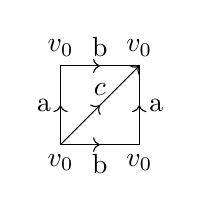
\begin{tikzpicture}[scale=0.5]
	\draw[->] (-5,0) node[below]{$v_0$}--(-4,0) node[below]{b};
	\draw[->] (-5,2) node[above]{$v_0$}--(-4,2) node[above]{b};
	\draw[->] (-5,0)--(-5,1) node[left]{a};
	\draw[->] (-3,0) node[below]{$v_0$}--(-3,1) node[right]{a};
	\draw[->] (-5,0)--(-4,1) node[above]{$c$};
	\draw[->] (-4,1)--(-3,2);
	\draw (-5,0)--(-3,0)--(-3,2) node[above]{$v_0$}--(-5,2)--cycle;
\end{tikzpicture}

	 Cellular and simplicial homology actually coincide. However we currently lack the framework for cellular homology}.

\begin{figure}
	
\parbox[c]{.5\linewidth}{\centering
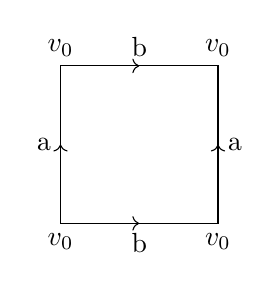
\begin{tikzpicture}
	\draw[->] (-5,0) node[below]{$v_0$}--(-4,0) node[below]{b};
	\draw[->] (-5,2) node[above]{$v_0$}--(-4,2) node[above]{b};
	\draw[->] (-5,0)--(-5,1) node[left]{a};
	\draw[->] (-3,0) node[below]{$v_0$}--(-3,1) node[right]{a};
	\draw (-5,0)--(-3,0)--(-3,2) node[above]{$v_0$}--(-5,2)--cycle;
\end{tikzpicture}}%
\parbox[c]{.5\linewidth}{\centering
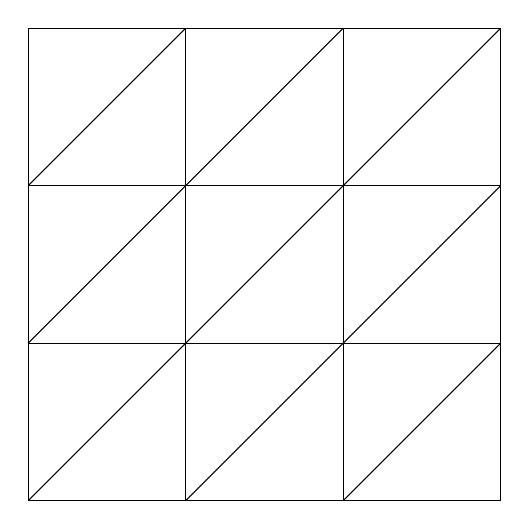
\begin{tikzpicture}
	\draw (0,0)--(6,0)--(6,6)--(0,6)--cycle;
	\draw (2,0)--(2,6);
	\draw (4,0)--(4,6);
	\draw (0,2)--(6,2);
	\draw (0,4)--(6,4);
	\draw (0,4)--(2,6);
	\draw (0,2)--(4,6);
	\draw (0,0)--(6,6);
	\draw (2,0)--(6,4);
	\draw (4,0)--(6,2);
\end{tikzpicture}	
}
\parbox[t]{.5\linewidth}{\captionsetup{width=.9\linewidth}
\caption{The fundamental polygon of the torus.\label{torus}}}%
\parbox[t]{.5\linewidth}{\captionsetup{width=.9\linewidth}\caption{A simplicial triangulation of the torus.\label{triangulation-torus}}}
\end{figure}

We see that the homology groups for the Sphere and the Torus do not agree in every dimension. Since homotopy equivalent spaces %TODO am i showing this for homotopy or homeomotphic
have isomorphic homology groups (we will show that later), we find that the sphere cannot be homotopy equivalent to the torus.

\item We will now consider the circle. This can be triangulated as an empty triangle, i.e.
\begin{center}
	
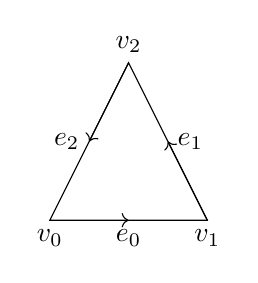
\begin{tikzpicture}
	\draw[->] (0,0)--(1,0) node[below]{$e_0$};
	\draw[->] (2,0)--(1.5,1)node[right]{$e_1$};
	\draw[->] (1,2)--(0.5,1)node[left]{$e_2$};
	\draw (0,0) node[below]{$v_0$}--(2,0) node[below]{$v_1$}--(1,2) node[above]{$v_2$}--cycle;
\end{tikzpicture}
\end{center}

We easily find 
\[
\partial_1=\begin{bmatrix}
-1&0&1\\1&-1&0\\0&1&-1
\end{bmatrix},\quad \partial_0\equiv 0
\]
Therefore,
\[H_1(\Sp^1)\simeq\Z/0\simeq\Z,\quad H_0(\Sp)\simeq\Z^3/\Z^2\simeq\Z
\]
\item 
Now that we have considered the circle, we might also be interested in the $2$-ball $B^2$. The triangulation is very easy this time. It is just one 2-dimensional simplex:
\begin{center}
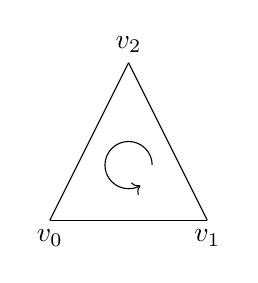
\begin{tikzpicture}
\draw[] (4,0) node[below]{$v_0$}--(6,0)node[below]{$v_1$};
\draw[] (6,0) -- (5,2) node[above]{$v_2$};
\draw[] (5,2)--(4,0);
%\draw (5,-1) node{$(v_0,v_1,v_2)$};	
\draw[->] (5.3,0.7)arc[start angle=0, end angle=300,radius=0.3cm];
\end{tikzpicture}

We find that $\partial_1$ and $\partial_0$ are the same as before and $\partial_2$ can be expressed as
\[
\partial_2=\begin{bmatrix}
1\\1\\1
\end{bmatrix}
\]
We then find
\[
H_2(B^2)=0,\quad H_1(B^2)=0,\quad H_0(B^2)=\Z
\]

\end{center}
	\end{enumerate}
\end{examples}


\section{\SH{} Groups with $\mathbb{Z}/2\mathbb{Z}$ Coefficients}

Let us remind ourselves of the definition for $p$-chains (Definition \ref{def-chain}):
\begin{quotation}
	Let $K$ be a simlicial complex. A \textbf{$p$-chain} on $K$ is a function $c$ from the set of oriented $p$-simplices of $K$ to the integers such that:
	\begin{enumerate}
		\item $c(\sigma)=-c(\sigma^\prime)$ if $\sigma$ and $\sigma^\prime$ are opposite orientations of the same simplex.
		\item $c(\sigma)=0$ for all but finitely many oriented $p$-simplices $\sigma$.
	\end{enumerate}
\end{quotation}

There is actually no reason (other than our familiarity with it) to restrict ourselves to the integers here. In fact, the same statements hold true for any abelian group $G$ and it can be helpful to consider other groups than the integers. To denote the change of our underlying group, we use the notation
\[
C_n(K;G)\qandq H_n(K;G)
\]
for the group of chains and the homology group of $K$ with coefficients in $G$.

Since the group of chains with integer coefficients $C_n(K;\Z)=C_n(K)$ merely consists of linear combinations of elementary chains with integer coefficients, there is a neat way to derive $C_n(K;G)$ if $C_n(K;\Z)$ is already known. We find that
\[
C_n(K;G)\simeq C_n(K;\Z)\otimes_\Z G,
\]
which leads to many interesting phenomena. The same holds for homology groups.



This might be a good time to remember the fundamental theorem of finitely generated abelian groups (such as the homology groups) as it can be found in Munkres' book \cite[see ][Theorem 4.3, p. 24]{mu}:
\begin{theorem}[The fundamental theorem of finitely generated abelian groups]
	Let $G$ be a finitely generated abelian group. Let $T$ be its torsion subgroup.Then there exists a free abelian subgroup $H$ of $G$ having finite rank such that $G=H\oplus T$. 
\end{theorem}

Since there is no possibility of torsion after taking the tensor product with a field of characteristic 0, we find that for any such field $\mathbb{K}$ the homology group with coefficients in $\mathbb{K}$ is a $\mathbb{K}$-vectorspace.

\section{Functoriality Property}
\section{Homotopy Invariance of \SH}

\printbibliography
\end{document}